\section{Introduction}\label{sec:intro}
Autoregressive Moving Average (ARMA) models are one of the main tools for modelling time series, specially with applications in economics and finance. The general ARMA model is described as a one-dimensional discrete system, where it is assumed that the user has access to the complete data $z_t$; this assumption eliminates the consideration of an observer in the ARMA model. This work ignores this assumption and considers an observer for ARMA models.


Let us consider a system that can be modelled through two independent ARMA processes, but the information available to the user is only one-dimensional, namely, there exists an observer such that it transforms the input from the two real ARMA models and it returns a linear combination of the data. The objetive is to desgin a filter (Kalman-based) such that we can obtain relevant estimations for the original ARMA models.

In order to illustrate the situation at hand, in Fig. \ref{fig:filter_scheme} we propose a general block diagram for the filter for the case of two ARMA models.


\begin{figure}[H]
  \centering
  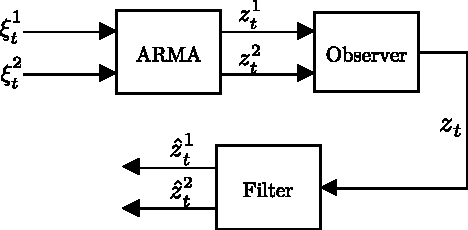
\includegraphics[scale=0.8]{files/arma_vadim.pdf}
  \caption{Filter scheme for observer-ARMA model.}
  \label{fig:filter_scheme}
\end{figure}
